\begin{frame}
    \frametitle{Implementation}
    \begin{itemize}
        \item Program structure:
        \begin{itemize}
            \item Read information files.
            \item Glut initialization.
            \item Display.
            \item Reshape.
        \end{itemize}
    \end{itemize}
\end{frame}

\begin{frame}
    \frametitle{Implementation}
    \begin{itemize}
        \item \texttt{GL\_POINTS}
    \end{itemize}
    \begin{figure}
        \begin{center}
           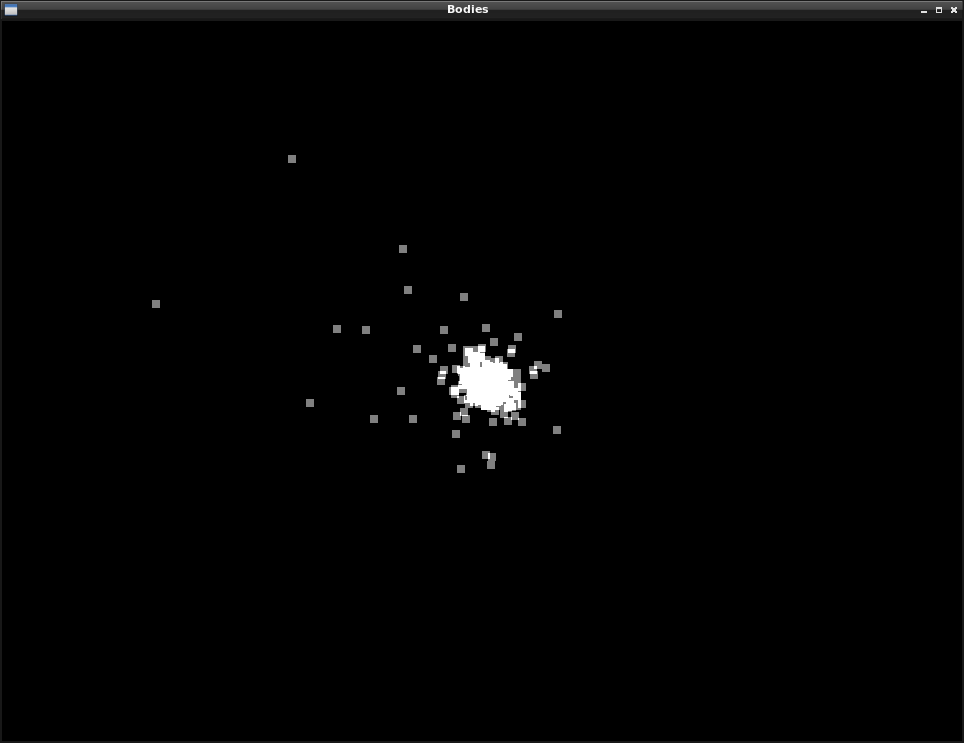
\includegraphics[width=0.6\textwidth]{img/bodies_sin_textura} 
        \end{center}
        \caption{Simple \texttt{GL\_POINTS} visualization (256)}
    \end{figure}
\end{frame}

\begin{frame}
    \frametitle{Implementation}
    \begin{itemize}
        \item \texttt{GL\_POINTS} + \texttt{GL\_TEXTURE\_2D}
    \end{itemize}
    \begin{figure}
        \begin{center}
           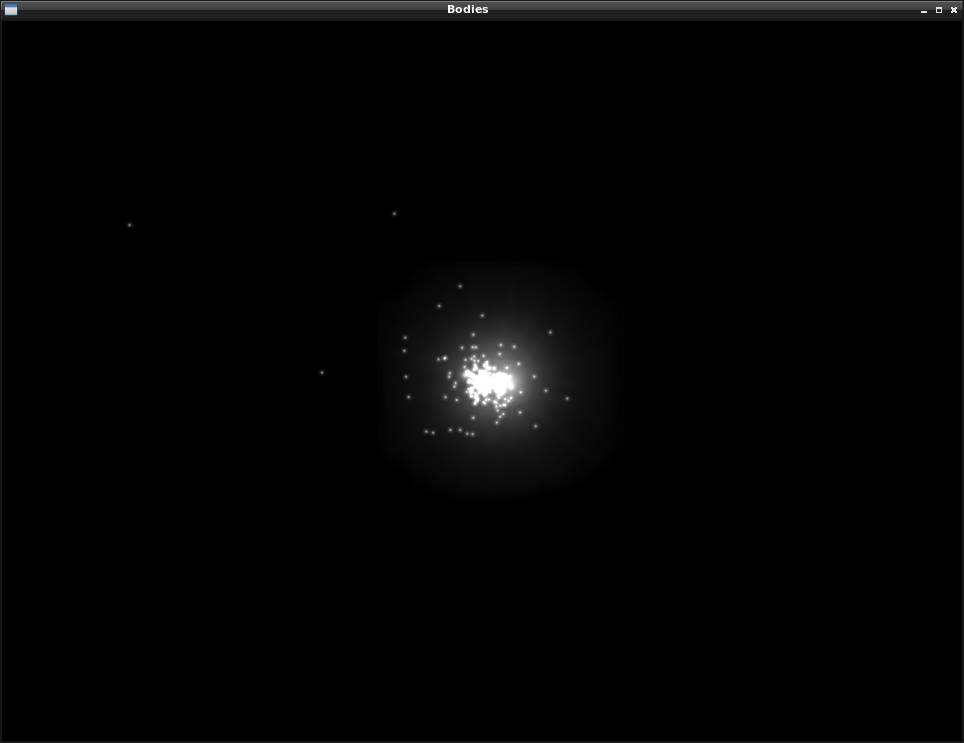
\includegraphics[width=0.6\textwidth]{img/bodies_con_textura} 
        \end{center}
        \caption{\texttt{GL\_POINTS} + \texttt{GL\_TEXTURE\_2D} visualization (256)}
    \end{figure}
\end{frame}

\begin{frame}
    \frametitle{Implementation}
    \begin{figure}
        \begin{center}
           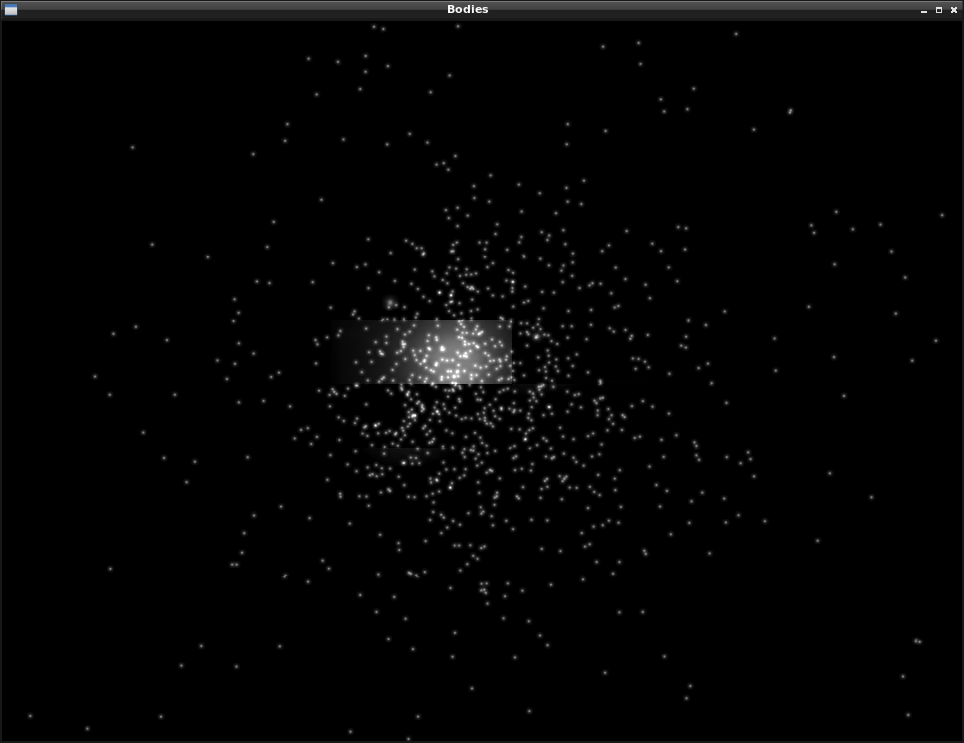
\includegraphics[width=0.7\textwidth]{img/bodies_con_textura_1024-2} 
        \end{center}
        \caption{Final visualization (1024)}
    \end{figure}
\end{frame}

\begin{frame}
    \frametitle{Implementation}
    \framesubtitle{Camera}
    \begin{figure}
        \begin{center}
           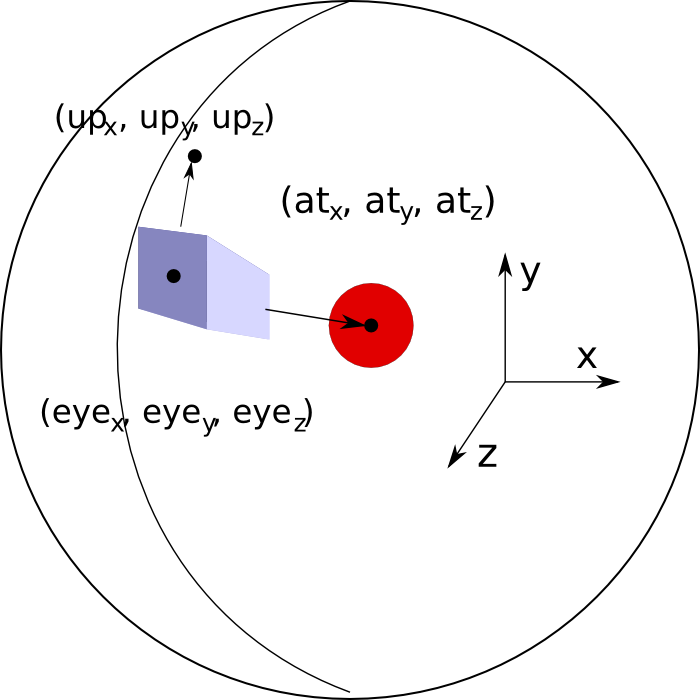
\includegraphics[width=0.5\textwidth]{img/camera} 
        \end{center}
        \caption{Camera movement using gluLookAt}
    \end{figure}
\end{frame}

\begin{frame}
    \frametitle{Implementation}
    \framesubtitle{Spherical coordinates}
    \begin{columns}
        \begin{column}{0.5\textwidth}
            \begin{eqnarray}
                (r, \theta, \varphi) \nonumber \\ \nonumber \\
                r = \sqrt{x^{2} + y^{2} + z^{2}} \nonumber\\
                \theta  = \arccos \left( \frac{z}{r}\right) \nonumber \\
                \varphi = \arccos \left( \frac{y}{x}\right) \nonumber
            \end{eqnarray}
        \end{column}
        \begin{column}{0.5\textwidth}
            \begin{eqnarray}
                (x, y, z) \nonumber \\ \nonumber \\
                x = r \cos{\varphi} \sin{\theta} \nonumber \\
                y = r \sin{\varphi} \sin{\theta} \nonumber \\
                z = r \cos{\theta}  \nonumber
            \end{eqnarray}
        \end{column}
    \end{columns}
\end{frame}
